\section{Introducción a los Números Naturales y Enteros}

La necesidad de contar objetos y animales genera la necesidad de asociarlos con números, los primeros conocidos son los Números Naturales cuya notación es $\mathbb{N}$:
\[ \mathbb{N}=\{ 1,2,\dots\} \]
Una de las propiedades de los naturales es que cada número tiene un siguiente $\operatorname{sig}(n)$, así el siguiente a $1$ es $2$, el siguiente de $5$ es $6$, y así sucesivamente, en general dado el número natural $n$ el siguiente será $n+1$.

Además de permitirnos contar, con estos números se pueden resolver algunas ecuaciones asociadas a una primera operación elemental, la adición, por ejemplo hallar el valor de $x$ que cumpla:
\[ x+3=5 \]
cuya solución es \fbox{$x=2$} pues al reemplazar la variable $x$ por $2$ en la ecuación, resulta: $\fbox{2}+3=5$. De la misma forma, la ecuación $5x=15$ tiene como solución $x=3$.

Sin embargo, al tratar de resolver esta otra ecuación:
\[ x+4=1 \]
Encontramos que NO tiene solución en los naturales, es decir que ningún natural satisface la ecuación puesto que la solución corresponde a $x=-3$, el inverso aditivo del número natural $3$, no obstante no hace parte de los naturales $(-3\notin\mathbb{N})$. Es necesario considerar un nuevo conjunto que incluya los naturales, sus inversos aditivos y el cero. Tal es el conjunto de los números enteros denotado por $\mathbb{Z}$:
\[ \mathbb{Z}=\{\dots -2,-1,0, 1,2,\dots\} \]

\section{Operaciones elementales}
A continuación se presentan las operaciones en los naturales y algunas de sus propiedades:

\subsection*{Suma}
La operación suma en los naturales no reviste mayor complejidad, en los enteros $\mathbb{Z}$, vamos a tener una convención, para sumar dos enteros del mismo signo se suman y se deja el signo de los dos, así por ejemplo $-2-3=-5$, ahora, si los enteros son de signos distintos, se realiza la resta normalmente y se coloca el signo del mayor, veamos, $-4+1$, se hace la resta $4-1=3$ y se coloca el signo del mayor así que el resultado es $-4+1=\fbox{-3}$, presentado en una recta lo que estamos haciendo se puede ver en la figura (\ref{fig:restaenteros}), partiendo de $0$, nos vamos $4$ unidades hacia la izquierda esto es $-4$ y luego una unidad hacia la derecha $+1$ después de los dos movimientos quedamos ubicados en $\fbox{-3}$ que es el resultado final:

\begin{figure}[ht]
\begin{center}
\caption{Resta de Enteros}\label{fig:restaenteros}
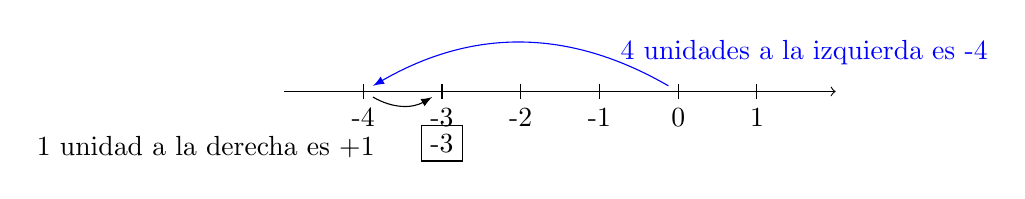
\begin{tikzpicture}[scale=1]
\draw[->] (-5.0,0.0) -- (2.0,0.0);
\foreach \x in {-4,-3,-2,-1,0,1} \draw (\x,0.1)--(\x,-0.1) node[below] {\x};
\node[below] at (-3,-0.3) {\fbox{-3}};
\node (B) at (0,0) {};
\node (M) at (-4,0) {};
\node (P) at (-3,0) {};
\draw[blue,->,>=latex] (B) to[bend right] (M);
\draw[->,>=latex] (M) to[bend right] (P);
\node[blue] at (1.6,0.5) {4 unidades a la izquierda es -4};
\node at (-6.0,-0.7) {1 unidad a la derecha es +1};
\end{tikzpicture}
\end{center}  
\end{figure}

\begin{ejemplo}[Adicional: Suma en la recta]
    Si tenemos $2 + (-5)$, partimos de 0, avanzamos 2 a la derecha y luego retrocedemos 5 a la izquierda. Llegamos a $-3$.
    \[ 2 + (-5) = -3 \]
\end{ejemplo}

\subsection*{Producto y División}
A continuación se presentan aspectos relevantes del producto y la división de naturales y enteros:

\begin{enumerate}
    \item \textbf{Múltiplo:} Dado un número natural $k$, se dice que $m$ es un múltiplo de $k$ si existe $n\in \mathbb{N}$ tal que $m=kn$, así por ejemplo $6$ es múltiplo de $2$ porqué existe el número $3\in \mathbb{N}$ tal que $6=2\times 3$. Si se multiplica un natural $k$ por todos y cada uno de los números naturales resulta un conjunto denominado ``múltiplos de $k$'' que lo notaremos $M(k)$, así por ejemplo si queremos hallar los múltiplos de $2$, éste se multiplica por cada uno de los naturales, se obtiene:
    \[ M(2)=\{ 2,\ 4,\ 6, \dots \} \]

    \item \textbf{Algoritmo de Euclides (Algoritmo de la división):} Si por ejemplo se quieren repartir $11$ objetos entre $4$ personas, el proceso se hace por medio de restas sucesivas. Los $11$ elementos son el ``dividendo'' $D$, serán repartidos equitativamente entre $4$ personas o grupos, lo llamaremos el ``divisor'' $d$, a la cantidad de objetos que se entreguen a cada persona lo denominamos el ``cociente'' $c$, y al número de elementos sobrantes, o aquellos con los que no se pueden completar grupos completos, se llamará el ``residuo'' $r$.
    
    En la figura (\ref{fig:divisionlarga}) se muestra un resumen del proceso:
    \begin{figure}[ht]
    \centering
    \opidiv[displayintermediary=all, voperation=top]{11}{4}
    \caption{División Larga.}\label{fig:divisionlarga}
    \end{figure}

    Vemos una representación gráfica de la división en la figura (\ref{fig:divisiongraph}), así para hacer $11\div 4$, a cada persona (círculos de la figura) le corresponden $2$ objetos osea el cociente, al tratar de repartir los tres objetos restantes vemos que no es posible darle a cada persona otro objeto adicional, ``pues alguien se quedaría con uno menos!!'', por ésta razón el resultado será que a cada persona le corresponden dos objetos y del total sobran $3$ elementos que corresponde con el residuo.
    
    \begin{figure}[ht]
    \begin{center}
    \caption{División por restas sucesivas.}\label{fig:divisiongraph}
    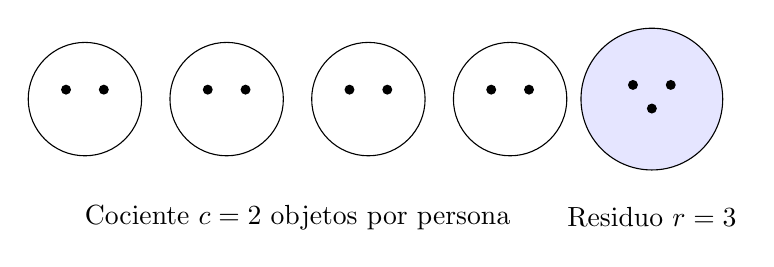
\begin{tikzpicture}[scale=0.6]
    \foreach \x in {-4,-1,2,5} {
        \draw (\x,0) circle [radius=1.2cm];
        \fill (\x-0.4,0.2) circle (3pt);
        \fill (\x+0.4,0.2) circle (3pt);
    }
    \node at (0.5, -2.5) {Cociente $c=2$ objetos por persona};
    \draw[fill=blue!10] (8,0) circle [radius=1.5cm];
    \node at (8, -2.5) {Residuo $r=3$};
    \fill (7.6,0.3) circle (3pt); \fill (8.0,-0.2) circle (3pt); \fill (8.4,0.3) circle (3pt);
    \end{tikzpicture}
    \end{center}  
    \end{figure}

    La división también la podemos representar como en (\ref{eq:divisionum}) así\footnote{En algunas ocasiones $2+\frac{3}{4}$ se escribe $2\frac{3}{4}$ y se lee ``dos enteros tres cuartos''.}:
    \begin{equation}\label{eq:divisionum}
         \frac{11}{4}=2+\frac{3}{4}
    \end{equation}

    En términos generales el algoritmo de Euclides se puede escribir como en (\ref{eq:euclides1}) y se leerá, dividendo ``D'' sobre divisor ``d'' es igual al cociente ``c'' más el residuo ``r'' sobre el divisor.
    \begin{equation}\label{eq:euclides1}
         \frac{D}{d}=c+\frac{r}{d}
    \end{equation}
     
    Al reescribir la ecuación (\ref{eq:euclides1}) se obtiene (\ref{eq:euclides}):
    \begin{equation}\label{eq:euclides}
        D=cd+r
    \end{equation}
    Así para el ejercicio que se había analizado de los $11$ objetos dividido entre $4$ personas, se puede escribir:
    \[ 11=2\times 4+3 \]

    \item \textbf{Divisibilidad:}
    Si el residuo de la división es cero $r=0$, la división es exacta y se obtiene $\frac{D}{d}=c$.
    Se dice que $d$ divide a $D$ si existe un entero $c$ tal que $D=dc$ y se denota por:
    \[ d|D \]
    $d$ es divisor de $D$, también se dice que $D$ es múltiplo de $d$. Si no existe tal entero se dice que $d$ no divide a $D$ y se escribe $d\not | D$.
    
    \textbf{Nota:} Nunca se puede hacer división por cero.

    Veamos un ejemplo $5|10$ pues existe el número $2$ tal que $10= 5\times 2$. También se puede afirmar que $10$ es múltiplo de $5$, mientras que por ejemplo $3$ no divide a $10$ osea $3\not| 10$ pues no existe un entero que al multiplicarlo por $3$ me resulte el número $10$.  

    \textbf{Conjunto de Divisores:} El conjunto de todos los divisores de un número natural $m$ se denomina ``Divisores de $m$'' y se nota $D(m)$, así por ejemplo los divisores de $12$ son:
    \[ D(12)=\{ 1,\ 2,\ 3,\ 4,\ 6,\ 12\} \]

    \textbf{Criterios de divisibilidad:} Dado un número natural $n$, se dice que:
    \begin{itemize}
        \item Un número es par si es múltiplo de $2$.
        \item Un número es divisible por $3$ si la suma de sus dígitos es múltiplo de $3$.
        \item Un entero es divisible por $5$ si termina en $0$ o en $5$.
    \end{itemize}

    \item \textbf{Número Primo:} Un número $p$ se dice que es primo, si su conjunto de divisores consta de dos números a saber, la unidad $1$ y el mismo número $p$, así: $D(p) = \{1,\ p\}$.
    Por ejemplo, $2$ es el único primo y además par.
    
    \begin{ejemplo}[Adicional: Primos gemelos]
        Dos números primos son gemelos si su diferencia es 2, como $(3,5)$, $(5,7)$ o $(11,13)$.
    \end{ejemplo}

    \item \textbf{Criba de Eratóstenes:} es un algoritmo que permite hallar todos los números primos menores que un número $m$ dado. En la tabla (\ref{tab:criba}) se muestra el procedimiento hasta 30.
%===========================================================
\begin{table}[ht]
\caption{Criba de Eratóstenes}\label{tab:criba}
\centering
\resizebox{12cm}{!}{%
\begin{tabular}{|c|c|c|c|c|c|l|l|l|l|}
\hline
$\not1$  &\textcolor{blue}{$2$}  & \textcolor{red}{$3$} & \textcolor{blue}{$\not4$}  & \textcolor{brown}{$5$} & \textcolor{blue}{$\not6$}  & 7  & \textcolor{blue}{$\not8$}  & \textcolor{red}{$\not9$}  & \textcolor{blue}{$\not{10}$} \\ \hline
11 & \textcolor{blue}{$\not12$} & 13 & \textcolor{blue}{$\not14$} & \textcolor{red}{$\not15$} & \textcolor{blue}{$\not16$} & 17 & \textcolor{blue}{$\not18$} & 19 & \textcolor{blue}{$\not20$} \\ \hline
\textcolor{red}{$\not21$} & \textcolor{blue}{$\not22$} & 23 & \textcolor{blue}{$\not24$} & \textcolor{brown}{$\not25$} & \textcolor{blue}{$\not26$} & \textcolor{red}{$\not27$} & \textcolor{blue}{$\not28$} & 29 & \textcolor{blue}{$\not30$} \\ \hline

\end{tabular}%
}
\end{table}
%=============================================
    \item \textbf{Teorema Fundamental de la Aritmética:} Todo número natural es primo o bien un producto único de números primos. Ejemplo: $6936=2^3\cdot 3\cdot 17^2$.
    
    Para descomponer 24:
    \begin{figure}[ht]
    \centering
    \begin{tabular}{c|c}
      24 & 2 \\ 12 & 2 \\ 6 & 2 \\ 3 & 3 \\ 1 & 
    \end{tabular}
    \caption{Descomposición factorial}\label{fig:primos}
    \end{figure}
    El resultado se escribe como $24=2^3\cdot 3$.

    \item \textbf{Máximo Común Divisor $\mathcal{MCD}$:} de dos números enteros $a$ y $b$ se denota por $\mathcal{MCD}(a,b)$.
    
    \textbf{Ejemplo:} Sean $a=12$, $b=48$.
    $D(12)=\{1,2,3,4,6,12\}$ y $D(48)=\{1,2,3,4,6,12,\dots\}$.
    $D(12)\cap D(48)=\{1,2,4,6,\fbox{12}\}$.
    $\mathcal{MCD}(12,48)=12$.

    \textbf{Teorema del Algoritmo Euclidiano:} Dados $b$ y $c$, aplicamos repetidamente la división.
    
    \textbf{Ejemplo:} Hallar $\mathcal{MCD}(963, 657)$.
    \begin{align}
        963 &= 657 \cdot 1 + 306 \label{eq:alg1}\\
        657 &= 306 \cdot 2 + 45 \label{eq:alg2}\\
        306 &= 45 \cdot 6 + 36 \label{eq:alg3}\\
        45 &= 36 \cdot 1 + 9 \label{eq:alg4}\\
        36 &= 9 \cdot 4 + 0 \nonumber
    \end{align}
    $\mathcal{MCD}(963,657)=9$. Expresado como combinación lineal (reversando):
    \begin{equation}
        9 = 657 \cdot 22 - 963 \cdot 15
    \end{equation}

    \item \textbf{Mínimo Común Múltiplo $\mathcal{MCM}$:} 
    \textbf{Ejemplo:} Calcular el $\mathcal{MCM}(10,14)$.
    \[ M(10)=\{10,20,\dots,\fbox{70},\dots,\fbox{140},\dots\} \]
    \[ M(14)=\{14,28,\dots,\fbox{70},\dots,\fbox{140},\dots\} \]
    $\mathcal{MCM}(10,14)=70$.

    \item \textbf{Método abreviado para hallar el $\mathcal{MCM}$ y $\mathcal{MCD}$:}
    En la tabla (\ref{tab:mcmmcd}) se ve el resumen para 160, 210 y 100.
    
    \begin{table}[ht]
    \centering
    \caption{Tabla para hallar $\mathcal{MCM}$ y $\mathcal{MCD}$}\label{tab:mcmmcd}
    \begin{tabular}{|c|c|c||c|}
    \hline
    160 & 210 & 100 & \textbf{2} \\
    80 & 105 & 50 & 2 \\
    40 & 105 & 25 & 2 \\
    20 & 105 & 25 & 2 \\
    10 & 105 & 25 & 2 \\
    5 & 105 & 25 & 3 \\
    5 & 35 & 25 & \textbf{5} \\
    1 & 7 & 5 & 5 \\
    1 & 7 & 1 & 7 \\
    1 & 1 & 1 & \\ \hline
    \end{tabular}
    \end{table}
    $\mathcal{MCD} = 2 \cdot 5 = 10$. $\mathcal{MCM} = 16800$.

    \item \textbf{Ejercicios:}
     \begin{enumerate}
         \item Aplicando el algoritmo Euclidiano encontrar el máximo común divisor de:
         a) 7469 y 2464 \hspace{3cm} b) 2689 y 4001
         \item Hallar el máximo común divisor de $1819$ y $3587$ y a continuación encontrar los enteros $x_0$, $y_0$ que satisfagan $1819x_0+3587y_0=g$
         \item Encontrar valores enteros $x$, $y$ que satisfagan $93x-81y=3$
     \end{enumerate}
\end{enumerate}

%==========================================================

\section{Ejercicios y Problemas Propuestos}

\subsection*{Nivel I: Mecánico y Procedimental}
\begin{enumerate}
    \item \textbf{Cálculo de $\mathcal{MCD}$ y $\mathcal{MCM}$:} 
    Para cada par de números, encuentre su máximo común divisor y su mínimo común múltiplo utilizando descomposición prima.
    \begin{enumerate}
        \item $a = 450, \quad b = 360$
        \item $a = 792, \quad b = 900$
        \item $a = 315, \quad b = 945$
    \end{enumerate}

    \item \textbf{Algoritmo de Euclides:}
    Utilice el algoritmo de Euclides para encontrar el $\mathcal{MCD}(a,b)$ y exprese el resultado como una combinación lineal de la forma $d = ax + by$ (Identidad de Bézout).
    \begin{enumerate}
        \item $a = 123, \quad b = 277$
        \item $a = 2024, \quad b = 76$
    \end{enumerate}

    \item \textbf{Divisibilidad:} 
    Sin realizar la división larga, determine si el número $N = 123,456,789$:
    \begin{enumerate}
        \item Es divisible por 3.
        \item Es divisible por 9.
        \item Es divisible por 11.
    \end{enumerate}
    \textit{Sugerencia: Use los criterios de divisibilidad explicados en clase.}
\end{enumerate}

\subsection*{Nivel II: Análisis y Aplicaciones}
\begin{enumerate}
    \setcounter{enumi}{3}
    \item \textbf{Problema de las Campanas:}
    Tres campanas en una iglesia tocan con intervalos distintos: la primera cada 45 minutos, la segunda cada 60 minutos y la tercera cada 90 minutos. Si todas sonaron juntas a las 8:00 a.m., ¿a qué hora volverán a sonar simultáneamente?

    \item \textbf{Problema de Baldosas:}
    Se desea cubrir el piso de una habitación rectangular de $420$ cm de largo por $480$ cm de ancho con baldosas cuadradas idénticas, sin cortar ninguna.
    \begin{enumerate}
        \item ¿Cuál es el mayor tamaño posible para el lado de cada baldosa?
        \item ¿Cuántas baldosas se necesitarán en total?
    \end{enumerate}

    \item \textbf{Ecuaciones Diofánticas Lineales:}
    Un granjero compró vacas a \$100 cada una y ovejas a \$17 cada una. Si gastó exactamente \$1800, ¿cuántos animales de cada tipo compró?
    \textit{Pista: Plantee la ecuación $100x + 17y = 1800$ y busque soluciones enteras no negativas.}
\end{enumerate}

\subsection*{Nivel III: Teórico y Demostraciones}
\textit{En esta sección se requiere justificar rigurosamente cada paso.}

\begin{enumerate}
    \setcounter{enumi}{6}
    \item \textbf{Propiedades del $\mathcal{MCD}$:}
    Demuestre que si $k$ es un entero positivo y $a, b \in \mathbb{Z}$, entonces:
    \[ \mathcal{MCD}(ka, kb) = k \cdot \mathcal{MCD}(a, b) \]

    \item \textbf{Números Primos:}
    Demuestre que si $p$ es un número primo y $p | ab$, entonces $p | a$ o $p | b$. 
    \textit{Sugerencia: Use la identidad de Bézout.}

    \item \textbf{Irracionalidad:}
    Demuestre por reducción al absurdo que $\sqrt{p}$ es irracional para cualquier número primo $p$. 
    \textit{Pista: Adapte la demostración clásica de $\sqrt{2}$.}

    \item \textbf{El Algoritmo de la División:}
    Sea $n$ un entero impar. Demuestre algebraicamente que $n^2 - 1$ es siempre divisible por 8.
    \textit{Pista: Un impar se escribe como $2k+1$. Analice $k$ par e impar.}
\end{enumerate}

\subsection*{Nivel IV: Retos (Desafío)}
\begin{enumerate}
    \setcounter{enumi}{10}
    \item \textbf{Primos de la forma $4k+3$:}
    Demuestre que existen infinitos números primos de la forma $4n+3$.
    \textit{Pista: Suponga que hay un número finito, $p_1, \dots, p_k$, y considere el número $N = 4p_1 \dots p_k - 1$.}

    \item \textbf{Sucesión de Fibonacci y $\mathcal{MCD}$:}
    Sea $F_n$ la sucesión de Fibonacci definida por $F_0=0, F_1=1, F_{n}=F_{n-1}+F_{n-2}$.
    Calcule $\mathcal{MCD}(F_{n}, F_{n+1})$ para cualquier $n \ge 1$.
    \textit{Pista: Aplique el algoritmo de Euclides a dos términos consecutivos.}
\end{enumerate}

\subsection*{Nivel V: Construcción y Programación (Opcional)}
\begin{enumerate}
    \setcounter{enumi}{12}
    \item \textbf{Algoritmo en Pseudocódigo:}
    Escriba un algoritmo (en pseudocódigo o diagrama de flujo) que reciba un número entero $N$ e imprima su descomposición en factores primos.
    \begin{itemize}
        \item Entrada: $60$
        \item Salida: $2, 2, 3, 5$
    \end{itemize}
\end{enumerate}

\section{El Conjunto de los Números Racionales $\mathbb{Q}$}

En la sección anterior se estudiaron las operaciones en naturales. Al realizar la división se obtuvieron términos de la forma $a/b$ o $a\div b$, cuya división podía ser exacta o no. De la misma forma, al intentar resolver ecuaciones de la forma $2x=3$, se encuentra que no tiene solución en los enteros, pues su solución es $x=\frac{3}{2}\notin\mathbb{Z}$. Así que es necesario entonces construir otro conjunto en el que halle este tipo de números, al cual denominamos el conjunto de los números \textbf{Racionales} $\mathbb{Q}$. Este conjunto contiene todos los enteros y los números de la forma $\frac{a}{b}$ o números fraccionarios donde $a,\ b\in\mathbb{Z}$, con $b\neq 0$, puesto que la división por cero produce una indeterminación. Los Racionales también se pueden identificar porque su desarrollo decimal es finito, o infinito periódico. Por ejemplo, el número Racional $\frac{2}{3}=0.66666\dots$, o $\frac{1}{2}=0.5$. El conjunto de los número Racionales se puede escribir como:

\begin{equation}
\mathbb{Q}=\left\{\frac{a}{b} \mid a,b\in\mathbb{Z}, b\neq 0\right\}.
\end{equation}

Así por ejemplo el conjunto $\{\dots -1.2,\ -0.8,\ -0.3333,\ 0,\ 0.5,\ 1.4,\ \dots\}\subset\mathbb{Q}$ es un subconjunto del conjunto de los números racionales, cuya característica es que su desarrollo decimal es finito o infinito periódico. A continuación presentamos algunas características importantes en el desarrollo de los números racionales, podemos decir que:

\begin{enumerate}
    \item \textbf{Significado:} Cuando estamos hablando de una fracción o una razón nos referiremos al cociente de dos números enteros $\frac{a}{b}$ siempre considerando que $b\neq 0$, se lee ``$a$ es a $b$'' o ``$a$ sobre $b$''. Siempre vamos a partir de una \textbf{unidad} o un valor que será nuestra \textbf{referencia} que se tomará como unidad; por ejemplo si tenemos una pizza, o un rectángulo, o un círculo, o un segmento se supone que es la unidad de medida patrón. Entonces el denominador $b$ representa el número de partes iguales en que se divide esa unidad, mientras que el numerador $a$ representa la cantidad que se toma o que se seleccionan del número total partido. Así por ejemplo $\frac{3}{4}$ significa que la unidad se partió en $4$ partes iguales y de esas se seleccionaron $3$. Veamos esto gráficamente: en la figura \ref{fig:fraccion01} se puede apreciar que la circunferencia se partió en $4$ partes iguales y se tomaron $3$ de ellas, por lo tanto la región sombreada representa $3/4$ de la circunferencia y la región en blanco representa $1/4$:

    \begin{figure}[ht]
    \caption{Representación Gráfica de la Fracción $\frac{3}{4}$}\label{fig:fraccion01}
    \centering
    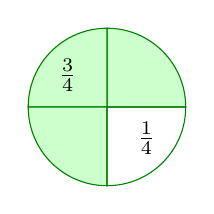
\begin{tikzpicture}
    \filldraw[fill=green!20,draw=green!50!black] (0,0) -- (1cm,0cm) arc [start angle=0, end angle=90, radius=1cm] -- cycle;
    \filldraw[fill=green!20,draw=green!50!black] (0,0) -- (0cm,1cm) arc [start angle=90, end angle=180, radius=1cm] -- cycle;
    \draw[fill=green!20,draw=green!50!black] (0,0) -- (-1cm,0cm) arc [start angle=180, end angle=270, radius=1cm] -- cycle;
    \draw[green!20,draw=green!50!black] (0,0) -- (0cm,-1cm) arc [start angle=270, end angle=360, radius=1cm] -- cycle;
    \node at (-0.5,0.4) {$\frac{3}{4}$};
    \node at (0.5,-0.4) {$\frac{1}{4}$};
    \end{tikzpicture}
    \end{figure}

    Si solo se utiliza una unidad, la fracción se llama \textbf{propia}; en el caso que acabamos de ver $3/4$ es una fracción propia en la cual el numerador es menor que el denominador y se dice que la fracción es menor que la unidad. Mientras que si se utiliza más de una unidad en su representación, esta se denomina fracción \textbf{impropia} y por supuesto resulta ser mayor que la unidad. Veamos un caso: representemos el número $5/3$. En este caso tomamos la unidad y la partimos en tres partes iguales, pero solo podemos tomar $3$ partes de esa unidad; se hace necesario entonces tomar otra unidad y partirla también en $3$ partes, de las cuales tomaremos $2$ para completar la fracción solicitada que se muestra en la figura \ref{fig:fraccion02}. En esa misma figura podemos ver que para representar la fracción se utilizó una unidad entera y $2/3$ de otra unidad; se puede escribir esta fracción como un número mixto $\frac{5}{3}=1\frac{2}{3}$ y se lee ``un entero dos tercios''.

    \begin{figure}[ht]
    \caption{Representación de la fracción impropia $5/3$}\label{fig:fraccion02}
    \centering
    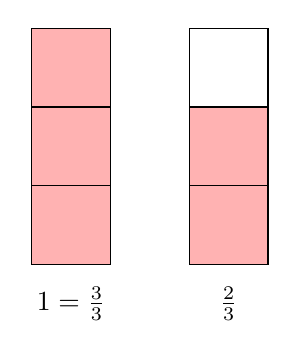
\begin{tikzpicture}
    \filldraw[red!30] (-2,-2) rectangle (-1,1);
    \draw (-2,-2) rectangle (-1,1);
    \draw (-2,-1)--(-1,-1);
    \draw (-2,0)--(-1,0);
    \filldraw[red!30] (0,-2) rectangle (1,-1);
    \draw (0,-2) rectangle (1,-1);
    \filldraw[red!30] (0,-1) rectangle (1,0);
    \draw (0,-1) rectangle (1,0);
    \draw (0,-2) rectangle (1,1);
    \node at (-1.5,-2.5) {$1=\frac{3}{3}$};
    \node at (0.5,-2.5) {$\frac{2}{3}$};
    \end{tikzpicture}
    \end{figure}

    Veamos que esto tiene relación directa con el algoritmo de Euclides, pues al hacer la división de $5$ entre $3$ se obtiene:
    \begin{center}
    \opidiv[displayintermediary=all, voperation=top]{5}{3}
    \end{center}
    Que lo escribimos como: 
    \[ \frac{5}{3}=1+\frac{2}{3} \]
    Una conclusión que podemos sacar de esta explicación es que si una unidad se divide en un número $b$ de partes y se toman $b$ partes, estamos tomando el equivalente a toda la unidad, así $\frac{3}{3}=1$, $\frac{5}{5}=1$. 

    \textbf{Propiedad de los racionales:} a cada racional $b\neq 0$ le corresponde otro racional $\frac{1}{b}$ tal que $b\cdot\frac{1}{b}=1$. Al número $\frac{1}{b}$ se le llama inverso multiplicativo del número $b$. En algunas ocasiones esto se escribe como la cancelación del número $b$ tanto en el numerador como en el denominador así $\cancel{b}\cdot{\frac{1}{\cancel{b}}}=1$. Así por ejemplo el inverso de $3$ es $\frac{1}{3}$ y cumple que $\cancel{3}\cdot\frac{1}{\not3}=1$, el inverso de $4$ es $\frac{1}{4}$ y cumple que $\cancel{4}\cdot\frac{1}{\not4}=1$, etc.

    \textbf{Representación sobre una recta:} Otra forma de representar los fraccionarios es sobre una recta infinita; se selecciona un punto arbitrario y se le asigna el número $0$, luego se selecciona un segmento (de cualquier longitud) que será nuestra unidad. Si por ejemplo queremos representar el fraccionario $1/2$ basta con dividir nuestra unidad en $2$ partes iguales y ubicar el segmento, allí estará el valor de la fracción, ver figura \ref{fig:fraccion03}.

    \begin{figure}[ht]
    \caption{Representación sobre una recta}\label{fig:fraccion03}
    \centering
    \begin{tikzpicture}
    \draw[->] (-1,0)--(2,0);
    \draw (0,0.1)--(0,-0.1);
    \node[below] at (0,0) {$0$};
    \draw (1,0.1)--(1,-0.1);
    \node[below] at (1,0) {$1$};
    \draw (0.5,0.1)--(0.5,-0.1);
    \node[above] at (0.5,0) {$\frac{1}{2}$};
    \end{tikzpicture}
    \end{figure}

    \item \textbf{Equivalencias:} los fraccionarios tienen distintas formas de escritura o de representación; en esta sección revisaremos algunas de esas representaciones equivalentes.

    \textbf{Fracciones equivalentes:} Una unidad se puede partir de distintas maneras. Así por ejemplo se puede representar el fraccionario $\frac{1}{2}$ partiendo la unidad en $2$ partes iguales y tomando una de esas partes como se puede apreciar en la figura \ref{fig:fraccion04}, pero al partir la misma unidad en $4$ partes iguales y tomar dos de esas partes se obtiene la misma región sombreada; el fraccionario equivalente es $\frac{2}{4}$, así podemos decir que $\frac{1}{2}=\frac{2}{4}$. Si partimos la unidad en $8$ partes y tomamos $4$ también podemos ver que representa la misma región sombreada, así $\frac{4}{8}=\frac{1}{2}$. En general diremos que dos fracciones son equivalentes si representan la misma región.

    \begin{figure}[ht]
    \caption{Fracciones Equivalentes a $\frac{1}{2}$}\label{fig:fraccion04}
    \centering
    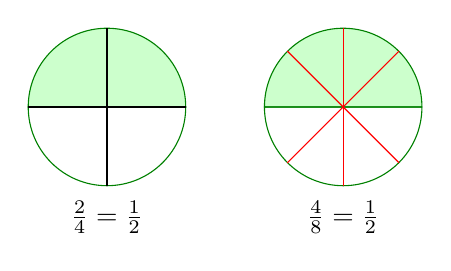
\begin{tikzpicture}
    \filldraw[fill=green!20,draw=green!50!black] (0,0) -- (1cm,0cm) arc [start angle=0, end angle=180, radius=1cm] -- cycle;
    \draw[green!20,draw=green!50!black] (0,0) -- (-1cm,0cm) arc [start angle=180, end angle=360, radius=1cm] -- cycle;
    \draw (0,0)--(0,1);
    \draw (0,0)--(-1,0);
    \draw (0,0)--(0,-1);
    \draw (0,0)--(1,0);
    \node at (0,-1.4) {$\frac{2}{4}=\frac{1}{2}$};
    
    \begin{scope}[shift={(3,0)}]
    \filldraw[fill=green!20,draw=green!50!black] (0,0) -- (1cm,0cm) arc [start angle=0, end angle=180, radius=1cm] -- cycle;
    \draw[green!20,draw=green!50!black] (0,0) -- (1cm,0cm) arc [start angle=0, end angle=-180, radius=1cm] -- cycle;
    \draw[red] (0,0)--(0.71,0.71);
    \draw[red] (0,0)--(0,1);
    \draw[red] (0,0)--(-0.71,0.71);
    \draw[red] (0,0)--(-0.71,-0.71);
    \draw[red] (0,0)--(0.0,-1.0);
    \draw[red] (0,0)--(0.71,-0.71);
    \node at (0,-1.4) {$\frac{4}{8}=\frac{1}{2}$};
    \end{scope}
    \end{tikzpicture}
    \end{figure}

    Es posible obtener fracciones equivalentes a una fracción dada si multiplicamos tanto el numerador como el denominador por una misma cantidad; las fracciones resultantes son equivalentes. A este proceso lo llamaremos \textbf{amplificación}, así por ejemplo: 
    \[ \frac{1}{2}=\frac{1\cdot 2}{2\cdot 2}=\frac{2}{4} \] 
    También lo podemos hacer por $4$ y resulta:
    \[ \frac{1}{2}=\frac{1\cdot 4}{2\cdot 4}=\frac{4}{8} \] 
    En realidad, podemos amplificar una fracción por cualquier número, resultando siempre una fracción equivalente.

    Para comprobar que dos fracciones digamos $\frac{a}{b}$ y $\frac{c}{d}$ son iguales, es posible hacer el producto cruzado: 
    \begin{equation}
    \frac{a}{b}=\frac{c}{d}\ \iff\ a\cdot d=c\cdot b 
    \end{equation}
    Así por ejemplo para determinar que $2/4$ equivale a $1/2$ podemos hacer $\frac{2}{4}=\frac{1}{2}$ y probar que $2\cdot 2=1\cdot 4=4$ y por tanto las fracciones son equivalentes.

    \textbf{Simplificación:} Cuando se tiene una fracción y tanto el numerador como el denominador se pueden escribir con su factorización prima, se pueden hacer las simplificaciones correspondientes y obtener una fracción equivalente a la fracción original. Así para el fraccionario $\frac{18}{24}$, descomponemos $18=2\cdot 3^2$ y $24=2^3\cdot 3$ y utilizando las propiedades de la potenciación resulta:
    \[ \frac{18}{24}=\frac{\cancel{2}\cdot 3^{\not2}}{2^{\not3}\cdot \cancel{3}}=\frac{3}{4} \]
    Que son equivalentes, pues al multiplicar en cruz se obtiene $18\cdot 4=72=3\cdot 24$.

    Al representar las fracciones sobre una recta, se está diciendo que el punto $1/2$ también se puede escribir como $\frac{\textcolor{red}{1}}{\textcolor{red}{2}}=\frac{\textcolor{blue}{2}}{\textcolor{blue}{4}}=\frac{\textcolor{brown}{3}}{\textcolor{brown}{6}}=\cdots$, como se puede ver en la figura \ref{fig:fraccion05}.

    \begin{figure}[ht]
    \caption{Fracciones Equivalentes}\label{fig:fraccion05}
    \centering
    \begin{tikzpicture}
    \draw[->] (-1,0)--(4,0);
    \draw (0,0.1)--(0,-0.1);
    \node[below] at (0,0) {$0$};
    \draw (2,0.1)--(2,-0.1);
    \node[below] at (2,0) {$1$};
    \draw (1,0.1)--(1,-0.1);
    \node at (1,0) {$\bullet$}; 
    \node at (1,0.5) {$\frac{\textcolor{red}{1}}{\textcolor{red}{2}}$};
    \node at (1,-0.5) {$\frac{\textcolor{blue}{2}}{\textcolor{blue}{4}}$};
    \node at (1,-1.1) {$\frac{\textcolor{brown}{3}}{\textcolor{brown}{6}}$};
    \node at (1,-1.6) {$\vdots$};
    \end{tikzpicture}
    \end{figure}

    Lo que indica que un punto sobre la recta tiene una cantidad infinita de representaciones.

    \textbf{Representación Decimal:} al hacer la división de un entero entre otro, puede ocurrir que la división sea exacta, por ejemplo al dividir $12\div 4 = 3$, pero puede ocurrir que la división no sea exacta como cuando tratamos de hacer $\frac{11}{4}$. En la figura \ref{fig:divisiondecimal01} se hacen los primeros pasos, de la misma forma que lo hacíamos en el algoritmo de Euclides:

    \begin{figure}[ht]
    \centering
    \opidiv[displayintermediary=all, voperation=top]{11}{4}
    \caption{División con Decimales (Inicio)}\label{fig:divisiondecimal01}
    \end{figure}

    Es claro que ningún número multiplicado por $4$ da $3$ como resultado, razón por la cual se agrega un $0$ al lado del $3$ y se coloca una coma en el cociente. Ahora se busca un número que multiplicado por $4$ esté cerca de $30$, este es $7$, y luego repetimos el proceso hasta obtener residuo cero, como se ve en la figura \ref{fig:divisiondecimal03}:

    \begin{figure}[ht]
    \centering
    \opidiv[displayintermediary=all, voperation=top]{11}{4}
    \caption{División con Decimales (Completa)}\label{fig:divisiondecimal03}
    \end{figure}
    
    Lo que quiere decir que $11/4$ equivale a $2,75$, y así cada uno de los racionales tiene una representación decimal; por ejemplo $\frac{1}{2}=0.5$, $\frac{2}{3}=0.66\bar{6}$ en el que la barra sobre el $6$ significa que el desarrollo decimal tiene infinitos números $6$. Así que podemos caracterizar los números racionales como aquellos números cuyo decimal sea finito, o infinito periódico. En resumen escribiremos que el conjunto de los números racionales $\mathbb{Q}$ se puede escribir como:
    \begin{align}
    \mathbb{Q} &= \left\{\frac{a}{b} \mid a,b\in\mathbb{Z}, b\neq 0\right\} \\
               &= \{\text{Números con desarrollo decimal finito o infinito periódico}\}
    \end{align}
    Todo número entero es un número racional, pues si $m\in\mathbb{Z}$ se puede escribir como $\frac{m}{1}=m$.

    \textbf{Porcentajes:} como las fracciones representan partes o porciones de una unidad, esa porción se puede escribir de otra forma; así por ejemplo $\frac{1}{2}=0.5$, que si se amplifica por $100$ resultando $0.5=\frac{50}{100}$ y por convención se utiliza que la fracción $\frac{1}{100}$ será equivalente al símbolo \%, así que $0.5=\frac{50}{100}=50\%$ lo que se lee como ``$50$ por ciento''. ¿Qué quiere decir esto? De una cantidad de objetos, digamos $20$, sacar el cincuenta por ciento equivale a multiplicar $(50\%)\cdot (20)$ que es igual a $\frac{50\cdot 20}{100}=\frac{1000}{100}=10$, es decir que el $50\%$ de $20$ son $10$ unidades, es decir la mitad.
    
    \begin{figure}[ht]
    \centering
    \caption{Interpretación gráfica del Porcentaje}\label{fig:porcentaje100}
    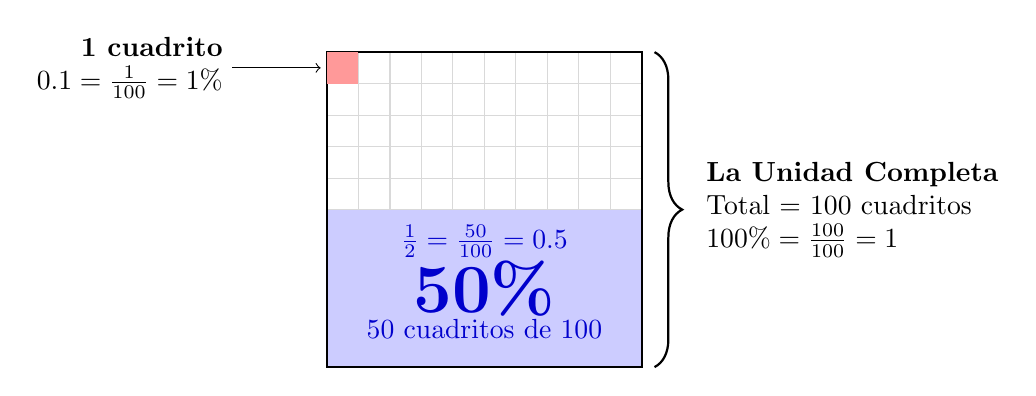
\begin{tikzpicture}[scale=0.8]
        % 1. La Cuadrícula base (10x10)
        % Dibujamos 100 cuadritos en gris muy suave
        \draw[step=0.5cm, gray!30, thin] (0,0) grid (5,5);
        
        % 2. Sombreado del 50% (50 cuadritos)
        % Llenamos la mitad inferior de azul
        \fill[blue!20] (0,0) rectangle (5,2.5);
        
        % 3. Borde grueso del TOTAL (El 100%)
        \draw[thick, black] (0,0) rectangle (5,5);
        
        % --- ANOTACIONES ---
        
        % Explicación de 1% (Un solo cuadrito)
        \fill[red!40] (0,4.5) rectangle (0.5,5); % Pintamos uno rojo
        \draw[<-] (-0.1, 4.75) -- (-1.5, 4.75) node[left, align=right] {\textbf{1 cuadrito}\\ $0.1=\frac{1}{100} = 1\%$};
        
        % Explicación del 50% (Área azul)
        \node[blue!80!black] at (2.5, 1.25) {\Huge \textbf{50\%}};
        \node[blue!80!black] at (2.5, 0.6) {50 cuadritos de 100};
        \node[blue!80!black] at (2.5, 2.0) {$\frac{1}{2}=\frac{50}{100} = 0.5$};
        
        % Explicación del 100% (Llave lateral)
        \draw[decorate, decoration={brace, amplitude=10pt, mirror}, thick] (5.2, 0) -- (5.2, 5) 
            node[midway, right=15pt, align=left] {\textbf{La Unidad Completa}\\ Total = 100 cuadritos\\ $100\% = \frac{100}{100} = 1$};

    \end{tikzpicture}
\end{figure}

    \item \textbf{Suma de Fraccionarios:} a continuación se presentan diversas opciones para realizar la suma de fracciones, dependiendo de si son \textbf{homogéneas} (mismo denominador) o \textbf{heterogéneas} (denominador distinto).

    \begin{enumerate}
        \item \textbf{Suma de Fracciones Homogéneas:} si tienen el mismo denominador, se suman los numeradores y se deja el mismo denominador:
        \begin{equation}
        \boxed{\frac{a}{b}+\frac{c}{b}=\frac{a+c}{b}}
        \end{equation}
        Por ejemplo: 
        \[ \frac{2}{5}+\frac{4}{5}=\frac{6}{5} \]

        \item \textbf{Suma de Fracciones Heterogéneas:} dadas dos fracciones con diferente denominador hay varias formas para realizar su suma:
        
        \textbf{Multiplicación en Cruz:}
        \begin{equation}
        \boxed{\frac{a}{b}+\frac{c}{d}=\frac{ad+bc}{bd}}
        \end{equation}
        Ejemplo:
        \[ \frac{3}{\textcolor{red}{4}}+\frac{\textcolor{brown}{2}}{\textcolor{blue}{5}}=\frac{3\cdot \textcolor{blue}{5}+\textcolor{brown}{2}\cdot \textcolor{red}{4}}{\textcolor{red}{4}\cdot \textcolor{blue}{5}}=\frac{15+8}{20}=\frac{23}{20} \]

        \textbf{Amplificando las fracciones:} para dejarlas con el mismo denominador.
        \[ \frac{2}{3}+4=\frac{2}{3}+\frac{4}{1}\cdot\frac{3}{3}=\frac{2}{3}+\frac{12}{3}=\frac{14}{3} \]

        \textbf{Utilizando el MCM:} Sumar $\frac{7}{90}$ con $\frac{13}{120}$. 
        $\mathcal{MCM}(90,120)=360$.
        \begin{equation*}
            \frac{7}{90}+\frac{13}{120}=\frac{7\cdot 4+13\cdot 3}{360}=\frac{28+39}{360}=\frac{67}{360}
        \end{equation*}
    \end{enumerate}
%===============================================================
\item \textbf{Multiplicación de Fraccionarios:} 
    Conceptualmente, multiplicar fracciones significa calcular una parte de otra parte. La palabra clave es ``\textbf{de}''.
    
    El algoritmo es directo: numerador por numerador y denominador por denominador.
    \begin{equation}
    \boxed{\frac{a}{b} \cdot \frac{c}{d} = \frac{a \cdot c}{b \cdot d}}
    \end{equation}
    \textbf{Ejemplo Numérico:} Multiplicar $\frac{2}{3}$ por $\frac{4}{5}$:
    \[ \frac{2}{3} \cdot \frac{4}{5} = \frac{2 \cdot 4}{3 \cdot 5} = \frac{8}{15} \]

    \textbf{Explicación Gráfica (Paso a paso):} 
    Vamos a visualizar la operación $\frac{2}{3} \cdot \frac{4}{5}$ (que se lee: ``dos tercios \textbf{de} cuatro quintos'') ver figura \ref{fig:multpasos}.
    
       \begin{figure}[ht]
    \centering
    \caption{Proceso gráfico de multiplicación con rejilla}\label{fig:multpasos}
    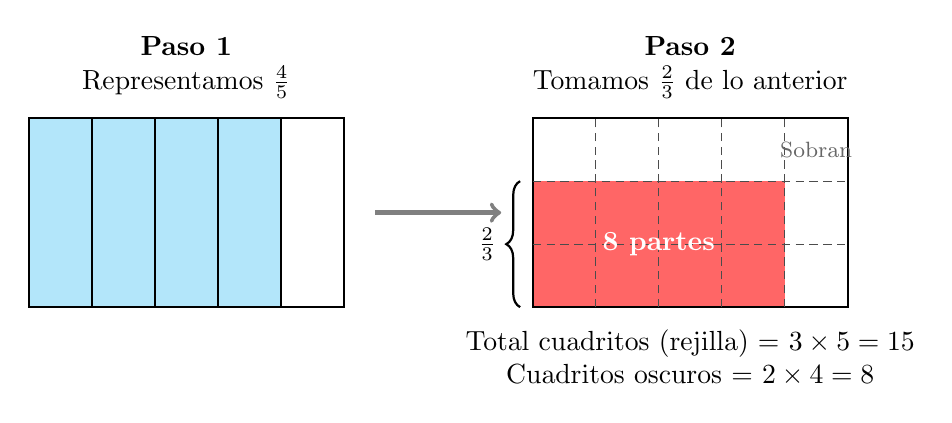
\begin{tikzpicture}[scale=0.8]
        % --- PASO 1: Representar 4/5 ---
        \node[align=center] at (2.5, 3.8) {\textbf{Paso 1}\\Representamos $\frac{4}{5}$};
        % Relleno Azul
        \fill[cyan!30] (0,0) rectangle (4,3);
        % Borde Unidad
        \draw[thick] (0,0) rectangle (5,3);
        % Divisiones Verticales (Quintos) - Sólidas
        \foreach \x in {1,2,3,4} \draw[thick] (\x,0) -- (\x,3);
        
        % Flecha de transición
        \draw[->, ultra thick, gray] (5.5, 1.5) -- (7.5, 1.5);

        % --- PASO 2: Cruzar con 2/3 y ver la rejilla ---
        \begin{scope}[shift={(8,0)}]
            \node[align=center] at (2.5, 3.8) {\textbf{Paso 2}\\Tomamos $\frac{2}{3}$ de lo anterior};
            
            % 1. Relleno Final (Intersección) - Más oscuro para destacar
            \fill[red!60] (0,0) rectangle (4,2);
            
            % 2. Borde Unidad
            \draw[thick] (0,0) rectangle (5,3);
            
            % 3. LA REJILLA COMPLETA (Líneas punteadas para visualizar el total)
            % Verticales (Quintos)
            \foreach \x in {1,2,3,4} \draw[densely dashed, black!70] (\x,0) -- (\x,3);
            % Horizontales (Tercios)
            \foreach \y in {1,2} \draw[densely dashed, black!70] (0,\y) -- (5,\y);
            
            % Etiquetas explicativas
            \draw[decorate, decoration={brace, amplitude=5pt}, thick] (-0.2, 0) -- (-0.2, 2) 
                node[midway, left=5pt] {$\frac{2}{3}$};
                
            \node[white, font=\bfseries] at (2,1) {8 partes};
            \node[black!60, font=\footnotesize] at (4.5, 2.5) {Sobran};
            
            % Conteo visual abajo
            \node[below, align=center] at (2.5, -0.2) {
                Total cuadritos (rejilla) = $3 \times 5 = 15$ \\
                Cuadritos oscuros = $2 \times 4 = 8$
            };
        \end{scope}
    \end{tikzpicture}
    \end{figure}
 
    \begin{enumerate}
        \item En el \textbf{Paso 1}, dividimos la unidad verticalmente en 5 partes y tomamos 4 (zona azul).
        \item En el \textbf{Paso 2}, dividimos horizontalmente en 3 partes y seleccionamos 2 filas (zona roja).
        \item El resultado es la zona roja, que contiene $4 \times 2 = 8$ cuadros.
        \item El total de cuadros en la rejilla nueva es $5 \times 3 = 15$.
    \end{enumerate}
    
    Por lo tanto:
    \[ \frac{2}{3} \cdot \frac{4}{5} = \frac{8}{15} \]



    \textbf{Ejemplo Numérico:} Multiplicar $\frac{3}{4}$ por $\frac{5}{7}$:
    \[ \frac{3}{4} \cdot \frac{5}{7} = \frac{3 \cdot 5}{4 \cdot 7} = \frac{15}{28} \]

%===============================================================
    
    \textbf{Recomendación (Simplificación previa):} En la multiplicación es muy útil simplificar cualquier numerador con cualquier denominador \textit{antes} de multiplicar, para evitar trabajar con números muy grandes.
    
    \textbf{Ejemplo con simplificación:} Multiplicar $\frac{4}{9} \cdot \frac{3}{10}$.
    \[ \frac{\textcolor{red}{4}}{\textcolor{blue}{9}} \cdot \frac{\textcolor{blue}{3}}{\textcolor{red}{10}} = \frac{\cancelto{2}{4} \cdot \cancelto{1}{3}}{\cancelto{3}{9} \cdot \cancelto{5}{10}} = \frac{2 \cdot 1}{3 \cdot 5} = \frac{2}{15} \]
    En este caso, simplificamos el 4 con el 10 (sacando mitad) y el 3 con el 9 (sacando tercera).
    
 \item \textbf{División de Fraccionarios:} 
    Conceptualmente, la división $\frac{a}{b} \div \frac{c}{d}$ responde a la pregunta: \textbf{¿Cuántas veces cabe la fracción $\frac{c}{d}$ dentro de la fracción $\frac{a}{b}$?}
    
    Existen dos métodos mecánicos principales para resolverla:
    
    \textbf{Método 1: Invertir y Multiplicar.} Se multiplica la primera fracción (dividendo) por el \textbf{inverso multiplicativo} de la segunda fracción (divisor).
    \begin{equation}
    \boxed{\frac{a}{b} \div \frac{c}{d} = \frac{a}{b} \cdot \frac{d}{c} = \frac{a \cdot d}{b \cdot c}}
    \end{equation}
    
    \textbf{Explicación Gráfica (El concepto de cabida):}
    Vamos a visualizar la división $\frac{3}{4} \div \frac{1}{8}$.
    
    Matemáticamente, aplicando la fórmula:
    \[ \frac{3}{4} \div \frac{1}{8} = \frac{3}{4} \cdot \frac{8}{1} = \frac{24}{4} = 6 \]
    Esto nos dice que $\frac{1}{8}$ cabe exactamente \textbf{6 veces} en $\frac{3}{4}$. Veámoslo:

        \begin{figure}[ht]
    \centering
    \caption{Visualización de $\frac{3}{4} \div \frac{1}{8}$ (¿Cuántos octavos caben?)}\label{fig:divfrac}
    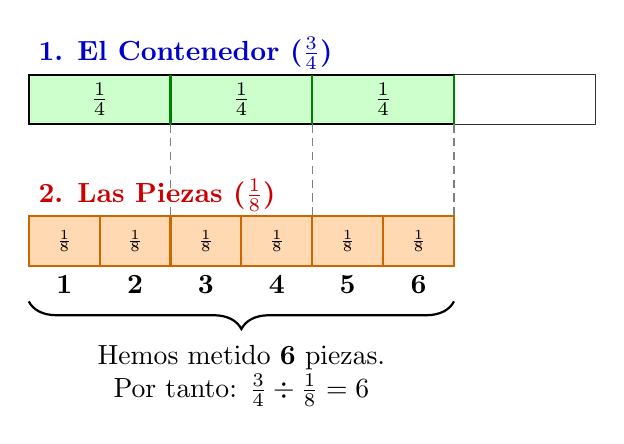
\begin{tikzpicture}[scale=0.9]
        % --- ESCALA: 8 unidades de ancho = 1 Entero ---
        
        % --- NIVEL 1: EL CONTENEDOR (3/4) ---
        \node[anchor=west, blue!80!black] at (0, 3.5) {\textbf{1. El Contenedor ($\frac{3}{4}$)}};
        
        % La Unidad completa fantasma (para referencia)
        \draw[black!80] (0,2.5) rectangle (8,3.2);
        
        % El 3/4 relleno
        \fill[green!20] (0,2.5) rectangle (6,3.2);
        \draw[thick] (0,2.5) rectangle (6,3.2);
        
        % Divisiones de cuartos
        \foreach \x in {2,4,6} \draw[thick, green!50!black] (\x,2.5) -- (\x,3.2);
        
        % Etiquetas de cuartos
        \node at (1, 2.85) {$\frac{1}{4}$};
        \node at (3, 2.85) {$\frac{1}{4}$};
        \node at (5, 2.85) {$\frac{1}{4}$};
        
        % --- LÍNEAS GUÍA (Muestran que 1/4 = 2/8) ---
        \foreach \x in {2,4,6} \draw[densely dashed, gray] (\x, 2.5) -- (\x, 1.2);

        % --- NIVEL 2: LAS PIEZAS (1/8) ---
        \node[anchor=west, red!80!black] at (0, 1.5) {\textbf{2. Las Piezas ($\frac{1}{8}$)}};
        
        % Dibujamos las 6 cajitas que caben
        \foreach \i in {0,1,2,3,4,5} {
            % Caja naranja
            \fill[orange!30] (\i,0.5) rectangle (\i+1,1.2);
            \draw[thick, orange!80!black] (\i,0.5) rectangle (\i+1,1.2);
            % Texto pequeño dentro
            \node[font=\tiny] at (\i+0.5, 0.85) {$\frac{1}{8}$};
            % Número de conteo abajo
            \node[font=\bfseries, below] at (\i+0.5, 0.5) {\number\numexpr\i+1};
        }
        
        % --- NIVEL 3: CONCLUSIÓN ---
        \draw[decorate, decoration={brace, amplitude=10pt, mirror}, thick] (0, 0) -- (6, 0) 
            node[midway, below=12pt, align=center] {
                Hemos metido \textbf{6} piezas.\\
                Por tanto: $\frac{3}{4} \div \frac{1}{8} = 6$
            };
            
    \end{tikzpicture}
    \end{figure}

    \textbf{Ejemplo General:} Para $\frac{2}{3} \div \frac{5}{7}$, aplicamos la regla:
    \[ \frac{2}{3} \div \frac{5}{7} = \frac{2}{3} \cdot \frac{7}{5} = \frac{14}{15} \]

    \textbf{Método 2: Ley de la Oreja (Producto de extremos y medios).} Se organiza la división como una "fracción de fracciones". El resultado es el producto de los extremos (los números de más arriba y más abajo) sobre el producto de los medios (los números internos).
    %==========================================================
        \begin{figure}[ht]
    \centering
    \begin{tikzpicture}
       \node (A) at (0,1.2) {$a$};
       \node (B) at (0,0.6) {$b$};
       \draw (A.south west) -- (A.south east); 
       
       \node (C) at (0,-0.6) {$c$};
       \node (D) at (0,-1.2) {$d$};
       \draw (C.south west) -- (C.south east); 
       
       \draw[thick] (-0.5,0) -- (0.5,0); 
       
       % CAMBIO CLAVE AQUÍ:
       % 'pos=0.1' pone el texto arriba (al inicio de la curva roja)
       \draw[red, ->] (A.east) to[bend left=80] node[pos=0.3, right] {Extremos ($a \cdot d$)} (D.east);
       
       % 'pos=0.9' pone el texto abajo (al final de la curva azul)
       \draw[blue, ->] (B.east) to[bend left=80] node[pos=0.9, right] {Medios ($b \cdot c$)} (C.east);
       
       \node at (5,0) {$= \dfrac{a \cdot d}{b \cdot c}$};
    \end{tikzpicture}
    \caption{Ley de la Oreja}\label{fig:leyoreja}
    \end{figure}


    %==========================================================    
    \textbf{Ejemplo:} $\dfrac{\frac{1}{2}}{\frac{3}{5}} = \frac{1 \cdot 5}{2 \cdot 3} = \frac{5}{6}$.
    
\end{enumerate}

\subsection*{Ejemplos Resueltos Adicionales}

\begin{ejemplo}
    Simplifique la fracción $\frac{84}{126}$ hasta su mínima expresión.
    
    \textbf{Solución:}
    Descomponemos numerador y denominador:
    $84 = 2^2 \cdot 3 \cdot 7$ y $126 = 2 \cdot 3^2 \cdot 7$.
    \[ \frac{84}{126} = \frac{2^2 \cdot 3 \cdot 7}{2 \cdot 3^2 \cdot 7} = \frac{2}{3} \]
\end{ejemplo}

\begin{ejemplo}
    Convierta el decimal periódico $0.333\dots$ a fracción.
    
    \textbf{Solución:}
    Sea $x = 0.333\dots$. Multiplicamos por 10: $10x = 3.333\dots$.
    Restamos $x$:
    \[ 10x - x = 3.333\dots - 0.333\dots \implies 9x = 3 \implies x = \frac{3}{9} = \frac{1}{3} \]
\end{ejemplo}

\subsection*{Ejercicios Propuestos}

\begin{enumerate}
    \item Realice las siguientes sumas y simplifique el resultado:
    \begin{enumerate}
        \item $\frac{3}{8} + \frac{1}{8}$
        \item $\frac{2}{5} + \frac{1}{3}$
        \item $\frac{5}{12} + \frac{7}{18}$
    \end{enumerate}
    
    \item Determine si las siguientes parejas de fracciones son equivalentes:
    \begin{enumerate}
        \item $\frac{3}{5}$ y $\frac{9}{15}$
        \item $\frac{4}{7}$ y $\frac{12}{20}$
    \end{enumerate}

    \item Un tanque se llena hasta sus $3/4$ partes. Si se sacan $1/5$ del total del tanque, ¿qué fracción del tanque queda llena?
\end{enumerate}

\subsection*{Ejemplos Resueltos Adicionales}

\begin{ejemplo}
    Simplifique la fracción $\frac{84}{126}$ hasta su mínima expresión.
    
    \textbf{Solución:}
    Descomponemos numerador y denominador:
    $84 = 2^2 \cdot 3 \cdot 7$ y $126 = 2 \cdot 3^2 \cdot 7$.
    \[ \frac{84}{126} = \frac{2^2 \cdot 3 \cdot 7}{2 \cdot 3^2 \cdot 7} = \frac{2}{3} \]
\end{ejemplo}

\begin{ejemplo}
    Convierta el decimal periódico $0.333\dots$ a fracción.
    
    \textbf{Solución:}
    Sea $x = 0.333\dots$. Multiplicamos por 10: $10x = 3.333\dots$.
    Restamos $x$:
    \[ 10x - x = 3.333\dots - 0.333\dots \implies 9x = 3 \implies x = \frac{3}{9} = \frac{1}{3} \]
\end{ejemplo}

\subsection*{Ejercicios Propuestos}

\begin{enumerate}
    \item Realice las siguientes sumas y simplifique el resultado:
    \begin{enumerate}
        \item $\frac{3}{8} + \frac{1}{8}$
        \item $\frac{2}{5} + \frac{1}{3}$
        \item $\frac{5}{12} + \frac{7}{18}$
    \end{enumerate}
    
    \item Determine si las siguientes parejas de fracciones son equivalentes:
    \begin{enumerate}
        \item $\frac{3}{5}$ y $\frac{9}{15}$
        \item $\frac{4}{7}$ y $\frac{12}{20}$
    \end{enumerate}

    \item Un tanque se llena hasta sus $3/4$ partes. Si se sacan $1/5$ del total del tanque, ¿qué fracción del tanque queda llena?
\end{enumerate}

\newpage % Salto de página recomendado para iniciar tema nuevo

\section{Números Irracionales y el Conjunto de los Reales \texorpdfstring{$\mathbb{R}$}{R}}

Todas las ecuaciones de la forma $bx=a$, con $a,b\in\mathbb{Z}$ y $b\neq 0$, tienen solución en $\mathbb{Q}$. Sin embargo, si la ecuación involucra potencias en la incógnita, esto no siempre ocurre. Por ejemplo, al intentar resolver la ecuación $x^2-2=0$, se demuestra que no existe ningún número racional $\frac{p}{q}$ que, elevado al cuadrado, resulte en $2$.

La solución formal a esta ecuación requiere la introducción de nuevos números. Al intentar escribir la solución positiva ($x=\sqrt{2}$) en notación decimal, encontramos que su desarrollo es infinito y \textbf{NO} periódico:
\[ \sqrt{2} \approx 1.41421356\dots \]

Este tipo de números conforma el conjunto de los \textbf{Números Irracionales}, simbolizado como $\mathbb{I}$. Se definen por tener una expansión decimal infinita no periódica. Algunos ejemplos notables son:

\begin{itemize}
    \item El número Pi: $\pi \approx 3.14159\dots$
    \item El número de Euler\footnote{En honor a Leonhard Euler. La pronunciación aproximada es ``Oiler''.}: $e \approx 2.71828\dots$
    \item La razón áurea\footnote{También conocida como divina proporción.}: $\phi = \frac{1+\sqrt{5}}{2} \approx 1.61803\dots$
\end{itemize}

Finalmente, definimos el conjunto de los \textbf{Números Reales} ($\mathbb{R}$) como la unión de los conjuntos Racional e Irracional:
\[ \mathbb{R} = \mathbb{Q} \cup \mathbb{I} \]

Geométricamente, estos números completan la recta numérica (propiedad de Completitud), de modo que a cada punto de la recta le corresponde un único número real, sin dejar ``huecos''.

\begin{figure}[ht]
\centering
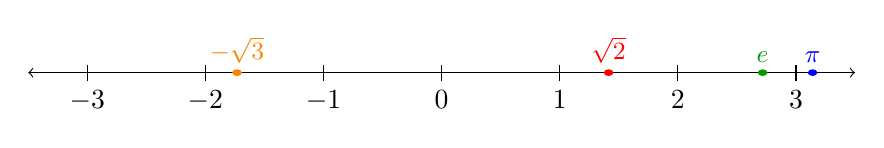
\begin{tikzpicture}[xscale=1.5]
    % Eje
    \draw[<->] (-3.5,0) -- (3.5,0);
    % Ticks enteros
    \foreach \x in {-3,-2,-1,0,1,2,3}
        \draw (\x,0.1) -- (\x,-0.1) node[below] {$\x$};
    
    % Irracionales notables (arriba del eje)
    \draw[red, fill] (1.414,0) circle (1pt) node[above] {\small $\sqrt{2}$};
    \draw[blue, fill] (3.141,0) circle (1pt) node[above] {\small $\pi$};
    \draw[green!60!black, fill] (2.718,0) circle (1pt) node[above] {\small $e$};
    \draw[orange, fill] (-1.732,0) circle (1pt) node[above] {\small $-\sqrt{3}$};
\end{tikzpicture}
\caption{Recta Real $\mathbb{R}$ con la ubicación aproximada de algunos irracionales.}\label{fig:rectareal}
\end{figure}

Una propiedad fundamental de los números reales es que son \textbf{densos}. A diferencia de los enteros, donde existe un antecesor y un sucesor definido, entre cualquier par de números reales existen infinitos números reales.

\begin{proposition}[Densidad de $\mathbb{R}$]
Si $a,b\in\mathbb{R}$ y $a<b$, entonces existe $c\in\mathbb{R}$ tal que $a<c<b$.
\end{proposition}

\begin{proof}
Tome el punto medio $c=\dfrac{a+b}{2}$. Como $a<b$, sumando $a$ a ambos lados obtenemos $2a < a+b \implies a < \dfrac{a+b}{2}$. Análogamente, sumando $b$ obtenemos $a+b < 2b \implies \dfrac{a+b}{2} < b$. Por lo tanto, $a<c<b$.
\end{proof}

\begin{corollary}
Entre cualesquiera $a<b$ existen infinitos números reales.
\end{corollary}

Aunque $\mathbb{R}$ permite resolver innumerables problemas, existen ecuaciones algebraicas simples sin solución real, como $x^2+1=0$ (ya que $x^2 \geq 0$ para todo real, implicando $x^2+1 \geq 1$).

Esto motiva la definición de la \textbf{unidad imaginaria} $i$, tal que $i^2 = -1$. A partir de ella se construye el conjunto de los \textbf{Números Complejos} ($\mathbb{C}$):
\[ \mathbb{C} = \{ a+ib \mid a,b \in \mathbb{R} \} \]
donde $a$ es la parte real y $b$ la parte imaginaria. Todo número real es también un número complejo (con $b=0$), lo que implica la contenencia $\mathbb{R} \subset \mathbb{C}$.

\begin{figure}[ht]
\centering
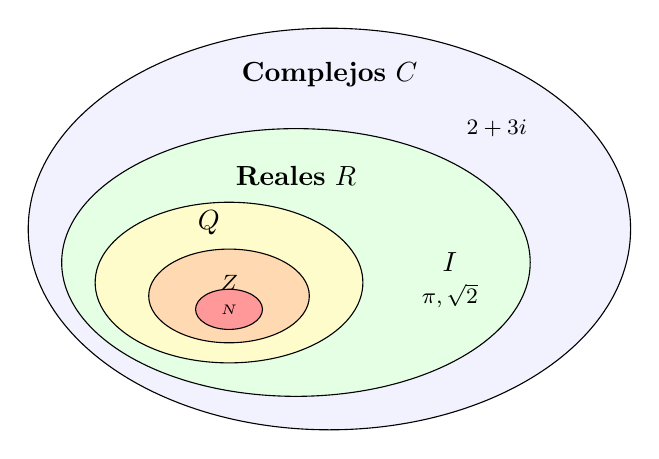
\begin{tikzpicture}[scale=0.85] % Escalado levemente para ajustar márgenes
    % Elipses
    \draw[fill=blue!5] (0,0) ellipse (4.5cm and 3cm);
    \node at (0,2.3) {\textbf{Complejos} $\mathbb{C}$};
    \node at (2.5,1.5) {\footnotesize $2+3i$};
    
    \draw[fill=green!10] (-0.5,-0.5) ellipse (3.5cm and 2cm);
    \node at (-0.5,0.8) {\textbf{Reales} $\mathbb{R}$};
    
    \draw[fill=yellow!20] (-1.5,-0.8) ellipse (2cm and 1.2cm);
    \node at (-1.8,0.1) {$\mathbb{Q}$};
    
    \draw[fill=orange!30] (-1.5,-1.0) ellipse (1.2cm and 0.7cm);
    \node at (-1.5,-0.8) {\footnotesize $\mathbb{Z}$};
    
    \draw[fill=red!40] (-1.5,-1.2) ellipse (0.5cm and 0.3cm);
    \node at (-1.5,-1.2) {\tiny $\mathbb{N}$};
    
    % Irracionales en la zona de R pero fuera de Q
    \node at (1.8,-0.5) {$\mathbb{I}$};
    \node at (1.8,-1.0) {\footnotesize $\pi, \sqrt{2}$};
\end{tikzpicture}
\caption{Jerarquía de los conjuntos numéricos.}\label{fig:diagrama_complejos}
\end{figure}

En este texto trabajaremos principalmente con el conjunto de los números reales, cuyas propiedades algebraicas y de orden constituyen la base del cálculo y el análisis matemático moderno.

\section{Propiedades de los Números Reales \texorpdfstring{$\mathbb{R}$}{R}}

En los números reales se definen dos operaciones, suma ($+$) y producto ($\cdot$)\footnote{Solo en esta sección utilizaremos $\cdot$; en el resto del libro, donde sea claro, se utilizará un punto o yuxtaposición para denotar el producto.}. Para cada una de ellas se cumplen las siguientes propiedades fundamentales.

\subsection*{Propiedades de la Suma}
Sean $a,b,c \in \mathbb{R}$:
\begin{enumerate}
    \item \textbf{Propiedad Clausurativa (S1):} $a+b \in \mathbb{R}$. La suma de reales es real.
    \item \textbf{Propiedad Conmutativa (S2):} $a+b = b+a$. El orden de los sumandos no altera el resultado.
    \item \textbf{Propiedad Asociativa (S3):} $(a+b)+c = a+(b+c)$. Podemos agrupar los sumandos de distintas formas.
    \item \textbf{Propiedad Elemento Neutro (S4):} Existe un real $0 \in \mathbb{R}$, llamado módulo de la suma, tal que para todo $a \in \mathbb{R}$:
    \[ a+0 = 0+a = a \]
    \item \textbf{Propiedad Invertiva (S5):} Para cada número $a \in \mathbb{R}$ existe otro número $-a \in \mathbb{R}$, llamado opuesto aditivo, tal que:
    \[ a+(-a) = 0 \]
\end{enumerate}

\subsection*{Propiedades del Producto}
Sean $a,b,c \in \mathbb{R}$:
\begin{enumerate}
    \item \textbf{Propiedad Clausurativa (P1):} $a\cdot  b \in \mathbb{R}$.
    \item \textbf{Propiedad Conmutativa (P2):} $a\cdot  b = b\cdot a$.
    \item \textbf{Propiedad Asociativa (P3):} $(a\cdot b)\cdot c = a\cdot(b\cdot c)$.
    \item \textbf{Propiedad del Elemento Inverso (P4):} Existe un real $1 \in \mathbb{R}$, llamado módulo del producto, tal que para todo $a \in \mathbb{R}$:
    \[ a\cdot 1 = 1\cdot a = a \]
    \item \textbf{Propiedad Invertiva (P5):} Para cada número $a \in \mathbb{R}$ con $a \neq 0$, existe otro número $a^{-1}$ o $\frac{1}{a} \in \mathbb{R}$, llamado inverso multiplicativo, tal que:
    \[ a \cdot \frac{1}{a} = 1 \]
\end{enumerate}

\subsection*{Propiedad Distributiva}
La propiedad que conecta la suma y el producto es la distributiva del producto respecto a la suma:
\[ a\cdot(b+c) = a\cdot b + a\cdot c \]
Esta propiedad es fundamental y se utiliza en dos direcciones:
\begin{itemize}
    \item \textbf{Productos Notables (Expansión):} De izquierda a derecha, distribuyendo el factor $a$.
    \item \textbf{Factorización (Factor Común):} De derecha a izquierda, extrayendo el factor $a$: $ab+ac = a(b+c)$.
\end{itemize}

\subsection*{Propiedades de la Igualdad}
Para resolver ecuaciones, usamos las siguientes propiedades de la igualdad. Sean $a,b,c \in \mathbb{R}$:
\begin{enumerate}
    \item \textbf{Uniformidad de la Suma (I1):} $a=b \iff a+c = b+c$.
    \item \textbf{Uniformidad del Producto (I2):} $a=b \iff a\cdot c = b\cdot c$, para todo $c \neq 0$.
    \item \textbf{Potenciación (I3):} Si $a=b$, entonces $a^n = b^n$ (para $n$ entero positivo).
\end{enumerate}

\section{Ejemplos Resueltos (Números Reales)}

\begin{ejemplo}
    Identifique a qué conjunto numérico pertenece cada número: $-5$, $2/3$, $\sqrt{7}$, $0$, $\pi$.
    
    \textbf{Solución:}
    \begin{itemize}
        \item $-5$: Entero ($\mathbb{Z}$), Racional ($\mathbb{Q}$), Real ($\mathbb{R}$).
        \item $2/3$: Racional ($\mathbb{Q}$), Real ($\mathbb{R}$).
        \item $\sqrt{7}$: Irracional ($\mathbb{I}$), Real ($\mathbb{R}$).
        \item $0$: Entero ($\mathbb{Z}$), Racional ($\mathbb{Q}$), Real ($\mathbb{R}$).
        \item $\pi$: Irracional ($\mathbb{I}$), Real ($\mathbb{R}$).
    \end{itemize}
\end{ejemplo}

\begin{ejemplo}
    Use las propiedades de los reales para despejar $x$ en la ecuación: $3(x+2) - 5 = 10$.
    
    \textbf{Solución:}
    \begin{align*}
        3(x+2) - 5 &= 10 & \text{(Ecuación original)} \\
        3x + 6 - 5 &= 10 & \text{(Propiedad Distributiva)} \\
        3x + 1 &= 10 & \text{(Suma de enteros)} \\
        3x + 1 + (-1) &= 10 + (-1) & \text{(Propiedad Uniforme Suma: sumar el opuesto)} \\
        3x &= 9 & \text{(Propiedad Invertiva Suma)} \\
        3x \cdot \frac{1}{3} &= 9 \cdot \frac{1}{3} & \text{(Propiedad Uniforme Producto: multiplicar por el inverso)} \\
        x &= 3 & \text{(Propiedad Invertiva Producto)}
    \end{align*}
\end{ejemplo}

\section{Ejercicios Propuestos (Números Reales)}

\begin{enumerate}
    \item Clasifique los siguientes números en Racionales ($\mathbb{Q}$) o Irracionales ($\mathbb{I}$):
    \begin{enumerate}
        \item $1.4142$ (Decimal finito)
        \item $\sqrt{2}$
        \item $3.1416$
        \item $\pi$
        \item $0.333\dots$
        \item $\frac{\sqrt{5}}{2}$
    \end{enumerate}

    \item Justifique cada paso de la solución de la ecuación $2x - 4 = 8$ nombrando la propiedad utilizada.

    \item ¿Es cierto que la suma de dos números irracionales es siempre irracional? (Sugerencia: Pruebe sumar $\sqrt{2}$ con $-\sqrt{2}$).

    \item Encuentre el inverso multiplicativo de los siguientes números:
    \begin{enumerate}
        \item $5$
        \item $-3/4$
        \item $0.5$
        \item $\pi$
    \end{enumerate}
    \item Encuentre dos o tres número racionales y dos o tres irracionales entre $0$ y $1$
\end{enumerate}


\section{Laboratorio de Matemáticas con Python}

En esta sección utilizaremos el lenguaje de programación \textbf{Python} para explorar los conceptos de números naturales, enteros y el algoritmo de la división vistos anteriormente. Python nos servirá como una herramienta para verificar propiedades y automatizar cálculos.

\subsection{Representación de Números ($\mathbb{N}$ y $\mathbb{Z}$)}
En matemáticas diferenciamos entre naturales ($\mathbb{N}$) y enteros ($\mathbb{Z}$). En Python, ambos se representan con el tipo de dato \texttt{int} (entero).

\begin{lstlisting}[caption=Asignación de variables]
# Un numero natural (n = 1)
n = 1 
print(n)

# Un numero entero negativo (z = -3)
z = -3
print(z)
\end{lstlisting}

\subsubsection*{Ejercicio Resuelto 1: El Sucesor}
\textbf{Problema:} Dado $n=5$, usar Python para encontrar su sucesor ($\operatorname{sig}(n) = n+1$).

\textbf{Solución en Python:}
\begin{lstlisting}
n = 5
sucesor = n + 1
print("El sucesor de", n, "es", sucesor)
# Salida: El sucesor de 5 es 6
\end{lstlisting}

\subsubsection*{Ejercicio Propuesto 1}
Define una variable \texttt{x} con el valor 10. Escribe un código que calcule e imprima el sucesor del sucesor de \texttt{x} (es decir, $x+2$).

\subsection{Operaciones Elementales y Signos}
Python respeta las reglas de los signos que vimos en la recta numérica. Por ejemplo, para calcular $-4 + 1$, Python realiza la operación automáticamente.

\begin{lstlisting}
resultado = -4 + 1
print(resultado)
# Salida: -3
\end{lstlisting}

\subsubsection*{Ejercicio Resuelto 2: Verificación de Ecuaciones}
\textbf{Problema:} Verificar si $x=2$ es la solución de la ecuación $x+3=5$.

\textbf{Solución:} Usamos el operador de comparación \texttt{==} que devuelve \texttt{True} (Verdadero) o \texttt{False} (Falso).

\begin{lstlisting}
x = 2
# Es x + 3 igual a 5?
verificacion = (x + 3 == 5)
print("Es x=2 la solucion?:", verificacion)
# Salida: Es x=2 la solucion?: True
\end{lstlisting}

\subsubsection*{Ejercicio Propuesto 2}
Usa Python para verificar si $x=3$ es la solución de la ecuación $x + 4 = 1$. ¿Qué resultado lógico (\texttt{True} o \texttt{False}) esperas obtener?

\subsection{Múltiplos y Listas}
El concepto de $M(k)$ (conjunto de múltiplos) se puede modelar en Python usando \textbf{listas} y la función \texttt{range()}.

\textbf{Ejemplo: Generar múltiplos de 2}\\
Matemáticamente: $M(2) = \{2, 4, 6, 8, 10, \dots\}$. En Python (primeros 5 múltiplos):

\begin{lstlisting}
# range(inicio, fin, paso)
# Empezamos en 2, vamos hasta 11 (para incluir el 10), paso de 2 en 2
multiplos_2 = list(range(2, 12, 2))
print("M(2) =", multiplos_2)
# Salida: M(2) = [2, 4, 6, 8, 10]
\end{lstlisting}

\subsubsection*{Ejercicio Resuelto 3: Múltiplos de 5}
\textbf{Problema:} Generar los primeros 3 múltiplos de 5.
\textbf{Solución:}
\begin{lstlisting}
# 5*1, 5*2, 5*3
k = 5
multiplos = [k*1, k*2, k*3]
print(multiplos)
# Salida: [5, 10, 15]
\end{lstlisting}

\subsubsection*{Ejercicio Propuesto 3}
Escribe un código que genere una lista con los múltiplos de 3, desde el 3 hasta el 15 inclusive.

\subsection{El Algoritmo de la División (Euclides)}
Como vimos en la teoría, la división tiene dos componentes principales cuando trabajamos con enteros: el \textbf{cociente} ($c$) y el \textbf{residuo} ($r$). Python tiene operadores específicos para esto:
\begin{itemize}
    \item \texttt{//} : División entera (obtiene $c$).
    \item \texttt{\%} : Módulo o residuo (obtiene $r$).
\end{itemize}

Recuerda la fórmula: $D = c \cdot d + r$.

\textbf{Ejemplo: Dividir 11 entre 4}
\begin{lstlisting}
D = 11  # Dividendo
d = 4   # Divisor

c = 11 // 4  # Cociente
r = 11 % 4   # Residuo

print("Cociente c:", c)
print("Residuo r:", r)

# Verificacion del algoritmo de Euclides
print("Comprobacion:", c * d + r) 
\end{lstlisting}

\subsubsection*{Ejercicio Resuelto 4: División Exacta}
\textbf{Problema:} Determinar si 6 es múltiplo de 2 usando el residuo.
\textbf{Solución:} Si el residuo es 0, la división es exacta.
\begin{lstlisting}
residuo = 6 % 2
if residuo == 0:
    print("6 es multiplo de 2")
else:
    print("6 NO es multiplo de 2")
\end{lstlisting}

\subsubsection*{Ejercicio Propuesto 4}
Calcula el cociente y el residuo de dividir 20 entre 3 utilizando Python. Luego, escribe una línea de código que verifique si se cumple que $20 = 3 \times c + r$.

\subsection*{Resumen de Operadores Python para esta sección}
\begin{center}
\begin{tabular}{|c|c|c|}
\hline
\textbf{Símbolo Matemático} & \textbf{Operador Python} & \textbf{Ejemplo} \\
\hline
$=$ (Asignación) & \texttt{=} & \texttt{x = 5} \\
\hline
$=$ (Igualdad) & \texttt{==} & \texttt{x == 5} \\
\hline
$+$ & \texttt{+} & \texttt{2 + 3} \\
\hline
$-$ & \texttt{-} & \texttt{4 - 1} \\
\hline
Cociente ($c$) & \texttt{//} & \texttt{11 // 4} \\
\hline
Residuo ($r$) & \texttt{\%} & \texttt{11 \% 4} \\
\hline
\end{tabular}
\end{center}

\section{Ejercicios de Profundización: Matemáticas Computacionales}

A continuación, se presentan problemas de nivel medio-avanzado que requieren dos etapas: una resolución analítica (lápiz y papel) para comprender la lógica, y una implementación computacional en Python para generalizar o verificar el resultado con números grandes.

\subsection*{Ejercicio 1: El Algoritmo de Euclides para el MCD}
En la sección anterior vimos que cualquier entero se puede escribir como $D = c \cdot d + r$. Euclides descubrió que el Máximo Común Divisor (MCD) de dos números $a$ y $b$ es el mismo que el MCD de $b$ y su residuo $r$. Es decir: 
\[ \text{mcd}(a, b) = \text{mcd}(b, r) \]
Este proceso se repite hasta que el residuo es 0.

\begin{enumerate}
    \item \textbf{Parte Teórica (Manual):} 
    Utiliza el algoritmo de la división por restas sucesivas (o división larga) para encontrar paso a paso el MCD de $a=252$ y $b=105$.
    
    \textit{Pista:} 
    \begin{itemize}
        \item Paso 1: $252 = 105 \times 2 + 42$ $\rightarrow$ Ahora busca mcd(105, 42).
        \item Paso 2: $105 = 42 \times \dots + \dots$
    \end{itemize}

    \item \textbf{Parte Computacional (Python):}
    Escribe un programa que automatice este proceso para cualquier par de números. Úsalo para encontrar el MCD de dos números grandes, por ejemplo: $123456$ y $7890$.
\end{enumerate}

\begin{lstlisting}[caption=Código propuesto para el Algoritmo de Euclides]
# Definimos los numeros
a = 123456
b = 7890

# Mientras el residuo no sea 0, seguimos dividiendo
while b > 0:
    r = a % b  # Calculamos el residuo
    a = b      # El divisor pasa a ser el nuevo dividendo
    b = r      # El residuo pasa a ser el nuevo divisor

print("El MCD es:", a)
\end{lstlisting}

\subsection*{Ejercicio 2: Aritmética Modular (El problema del calendario)}
El operador módulo (\texttt{\%}) nos dice "lo que sobra" después de completar grupos. Esto es la base de los calendarios (ciclos de 7 días). Imaginemos que numeramos los días: Lunes=0, Martes=1, ..., Domingo=6.

\begin{enumerate}
    \item \textbf{Parte Teórica (Manual):} 
    Si hoy es Lunes (0), ¿qué día de la semana será dentro de $100$ días? Resuélvelo usando la operación residuo:
    \[ \text{Día final} = ( \text{Día actual} + \text{Días transcurridos} ) \mod 7 \]
    
    \item \textbf{Parte Computacional (Python):}
    Python puede manejar enteros arbitrariamente grandes (cosa que las calculadoras normales no pueden). Escribe un script para determinar qué día de la semana será dentro de $10^{50}$ (un 1 seguido de 50 ceros) días.
\end{enumerate}

\begin{lstlisting}[caption=Calculando días en el futuro lejano]
dias_semana = ["Lunes", "Martes", "Miercoles", "Jueves", "Viernes", "Sabado", "Domingo"]

dia_actual = 0  # Lunes
dias_a_sumar = 10**50 # 10 elevado a la 50

# Aplicamos modulo 7
indice_final = (dia_actual + dias_a_sumar) % 7

print("Dentro de 10^50 dias sera:", dias_semana[indice_final])
\end{lstlisting}

\subsection*{Ejercicio 3: La Conjetura de Collatz ($3n+1$)}
Esta es una famosa conjetura matemática no resuelta. Toma cualquier número entero positivo $n$:
\begin{itemize}
    \item Si $n$ es par, divídelo entre 2: $n \to n/2$.
    \item Si $n$ es impar, multiplícalo por 3 y suma 1: $n \to 3n + 1$.
\end{itemize}
La conjetura dice que, sin importar con qué número empieces, eventualmente llegarás a 1.

\begin{enumerate}
    \item \textbf{Parte Teórica (Manual):} 
    Calcula manualmente la secuencia para $n=6$. Deberías obtener una serie de números hasta llegar al 1.
    
    \item \textbf{Parte Computacional (Python):}
    Escribe un programa que cuente cuántos pasos toma llegar a 1 para un número inicial $n = 27$. (Nota: El 27 tarda bastantes pasos, ¡es tedioso hacerlo a mano!).
\end{enumerate}

\begin{lstlisting}[caption=Simulación de la Conjetura de Collatz]
n = 27
pasos = 0

print("Secuencia para 27:")
while n != 1:
    if n % 2 == 0:     # Si es par
        n = n // 2     # Division entera
    else:              # Si es impar
        n = 3 * n + 1
    pasos = pasos + 1
    # Imprimimos en la misma linea para ahorrar espacio
    print(n, end=", ") 

print("\n\nTotal de pasos:", pasos)
\end{lstlisting}
